% Slide 28: Density-based Clustering
\begin{frame}{خوشه‌بندی مبتنی بر چگالی}{\lr{Density-based Clustering}}
  \begin{columns}[T]
    \begin{column}{0.54\textwidth}
      \begin{itemize}
        \setlength{\itemsep}{6pt}
        \item \textbf{محدودیت‌های کا-میانگین در کاربردهای پیچیده:}
        \begin{itemize}
          \setlength{\itemsep}{3pt}
          \item \textbf{چالش ۱: اشکال غیرکروی و دلخواه} \lr{(Non-globular shapes)}؛ کا-میانگین تنها خوشه‌های کروی محدب را به درستی می‌یابد.
          \item \textbf{چالش ۲: داده‌های پرت و نویزها} \lr{(Outliers / Noise points)}؛ کا-میانگین تمام نقاط را به زور در خوشه‌ها قرار می‌دهد.
        \end{itemize}
        \item \textbf{راه‌حل:} تعریف خوشه‌ها بر اساس پیوستگی نواحی با \textbf{چگالی بالا} و تفکیک آن‌ها توسط نواحی کم‌چگال.
      \end{itemize}
    \end{column}
    \begin{column}{0.44\textwidth}
      \begin{center}
        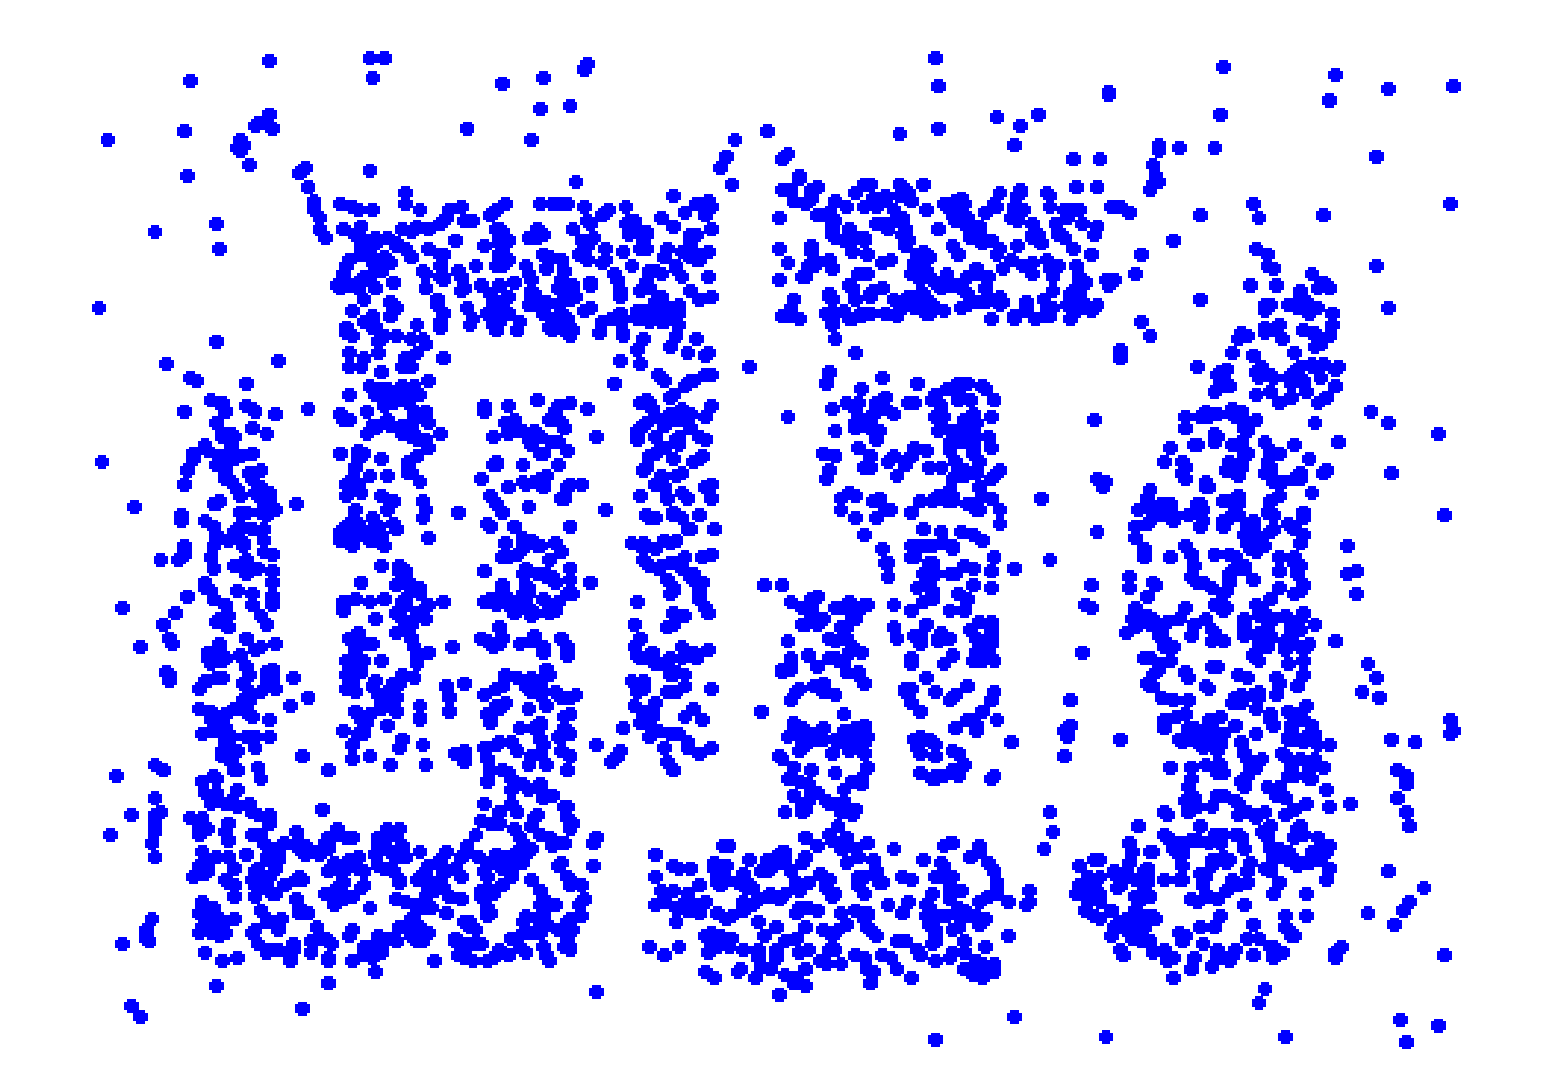
\includegraphics[width=\textwidth,height=4.6cm,keepaspectratio]{images/slide28_density_clusters.png}
      \end{center}
    \end{column}
  \end{columns}
\end{frame}

% Slide 29: DBSCAN Concepts
\begin{frame}{مفاهیم پایه الگوریتم \lr{DBSCAN}}{\lr{DBSCAN: Density-Based Spatial Clustering}}
  \begin{itemize}
    \setlength{\itemsep}{5pt}
    \item \textbf{تعریف چگالی:} تعداد نقاط موجود درون یک شعاع مشخص به نام \textbf{اپسیلون} ($\epsilon$ یا \lr{Eps}).
    \item الگوریتم نقاط داده را به \textbf{سه دسته} متمایز تقسیم می‌کند:
    \begin{itemize}
      \setlength{\itemsep}{4pt}
      \item \textbf{نقطه هسته:} \lr{(Core Point)} نقطه‌ای که در همسایگی شعاع $\epsilon$ آن، حداقل به تعداد مشخصی نقطه \lr{(MinPts)} وجود داشته باشد (خود نقطه نیز شمرده می‌شود). این نقاط بخش درونی خوشه‌ها را تشکیل می‌دهند.
      \item \textbf{نقطه مرزی:} \lr{(Border Point)} نقطه‌ای که تعداد همسایگان آن در شعاع $\epsilon$ کمتر از \lr{MinPts} است، اما در همسایگی یک نقطه هسته قرار دارد.
      \item \textbf{نقطه نویز / پرت:} \lr{(Noise Point)} هر نقطه‌ای که نه نقطه هسته باشد و نه نقطه مرزی.
    \end{itemize}
  \end{itemize}
\end{frame}

% Slide 30: Examples of Core, Border, and Noise
\begin{frame}{نمونه‌هایی از نقاط هسته، مرزی و نویز}{\lr{Examples of Core, Border, and Noise Points}}
  \begin{columns}[T]
    \begin{column}{0.48\textwidth}
      \begin{itemize}
        \setlength{\itemsep}{6pt}
        \item \textbf{تنظیم پارامترها:}
        \begin{itemize}
          \item $\text{MinPts} = 5$
          \item $\text{Eps} (\epsilon) = 1$
        \end{itemize}
        \item \textbf{نقطه هسته:} \lr{(Core)} درون دایره شعاع ۱ حداقل ۵ همسایه دارد.
        \item \textbf{نقطه مرزی:} \lr{(Border)} کمتر از ۵ همسایه دارد، اما در شعاع ۱ یک هسته قرار گرفته است.
        \item \textbf{نقطه نویز:} \lr{(Noise)} تنها افتاده و هیچ نقطه هسته‌ای در نزدیکی آن نیست.
      \end{itemize}
    \end{column}
    \begin{column}{0.5\textwidth}
      \begin{center}
        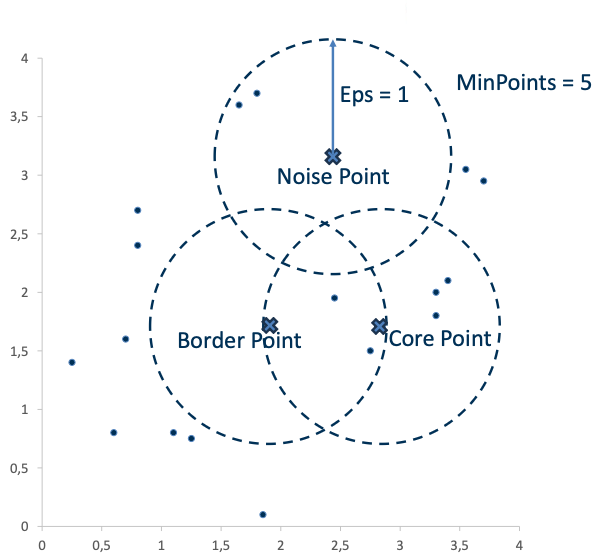
\includegraphics[width=\textwidth,height=4.8cm,keepaspectratio]{images/slide30_dbscan_points_user.png}
      \end{center}
    \end{column}
  \end{columns}
\end{frame}

% Slide 31: Core, Border, Noise Illustration
\begin{frame}{شناسایی انواع نقاط در مجموعه داده}{\lr{Point Types: Core, Border, and Noise}}
  \begin{center}
    {\fontsize{10}{12}\selectfont\color{mannheimblue}\textbf{تفکیک نقاط داده بر اساس چگالی محلی}}\\[0.2cm]
  \end{center}
  \begin{columns}[T]
    \begin{column}{0.48\textwidth}
      \begin{center}
        \textbf{نقاط اصلی داده‌ها \lr{(Original Points)}}\\[0.15cm]
        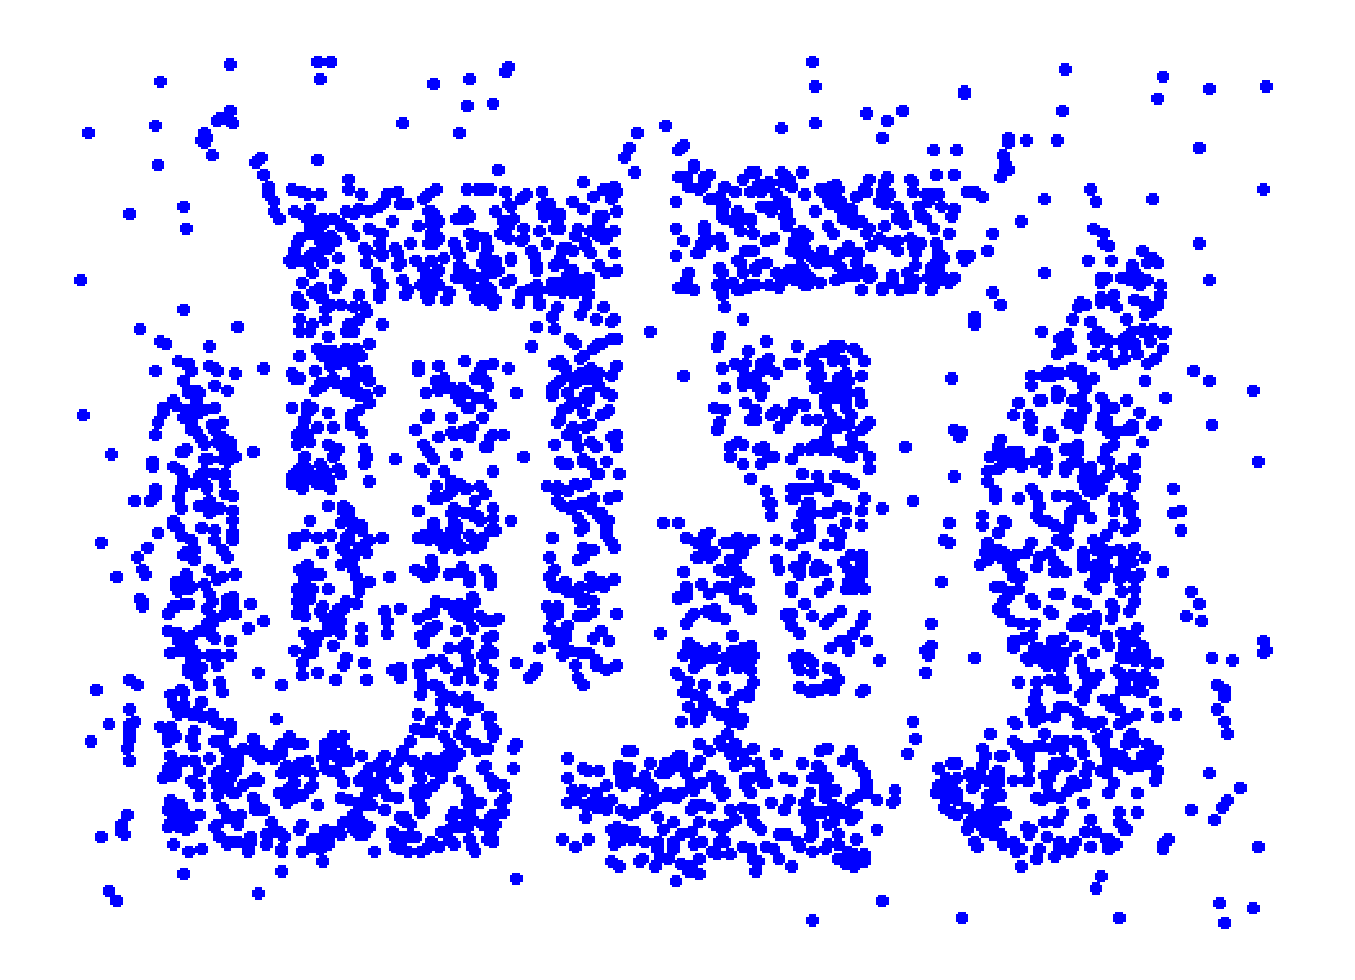
\includegraphics[width=\textwidth,height=4.0cm,keepaspectratio]{images/slide31_dbscan_diagram1.png}
      \end{center}
    \end{column}
    \begin{column}{0.48\textwidth}
      \begin{center}
        \textbf{دسته‌بندی نقاط به هسته، مرزی و نویز}\\[0.15cm]
        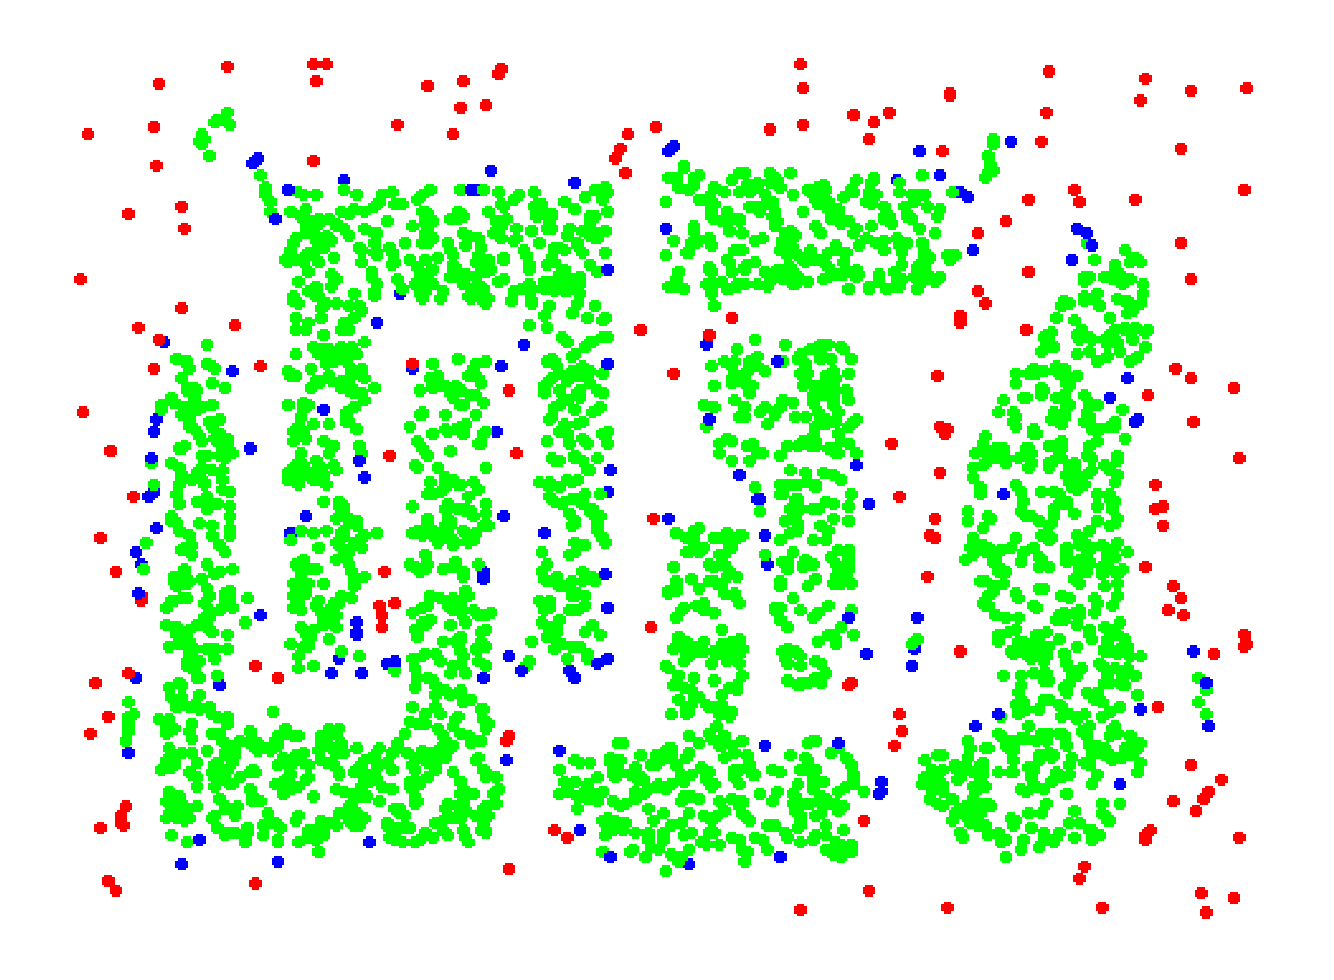
\includegraphics[width=\textwidth,height=4.0cm,keepaspectratio]{images/slide31_dbscan_diagram2.png}
      \end{center}
    \end{column}
  \end{columns}
\end{frame}

% Slide 32: DBSCAN Algorithm
\begin{frame}{الگوریتم خوشه‌بندی \lr{DBSCAN}}{\lr{The DBSCAN Algorithm}}
  \begin{itemize}
    \setlength{\itemsep}{3pt}
    \item ۱. شناسایی و حذف تمامی نقاط نویز \lr{(Noise Points)}.
    \item ۲. تشکیل خوشه‌ها با رشد زنجیره‌ای بر روی نقاط باقی‌مانده (هسته و مرزی).
  \end{itemize}

  \vspace{0.15cm}
  \begin{latin}
    \begin{minipage}{\textwidth}
      \fcolorbox{codeborder}{codebg}{%
        \begin{minipage}{0.96\textwidth}
          {\fontsize{7.2}{9.6}\selectfont\ttfamily
          \textbf{current\_cluster\_label} $\leftarrow 1$\\[0.1cm]
          \textbf{for} all core points \textbf{do}\\
          \quad \textbf{if} the core point has no cluster label \textbf{then}\\
          \quad\quad \textbf{current\_cluster\_label} $\leftarrow$ \textbf{current\_cluster\_label} $+ 1$\\
          \quad\quad Label the current core point with cluster label \textbf{current\_cluster\_label}\\
          \quad \textbf{end if}\\
          \quad \textbf{for} all points in the \textit{Eps}-neighborhood, except the point itself \textbf{do}\\
          \quad\quad \textbf{if} the point does not have a cluster label \textbf{then}\\
          \quad\quad\quad Label the point with cluster label \textbf{current\_cluster\_label}\\
          \quad\quad\quad \textcolor{mannheimteal}{\# Perform recursion for all points in the Eps-neighborhood}\\
          \quad\quad \textbf{end if}\\
          \quad \textbf{end for}\\
          \textbf{end for}
          }
        \end{minipage}%
      }
    \end{minipage}
  \end{latin}
\end{frame}

% Slide 33: Clustering Result
\begin{frame}{خوشه‌های نهایی الگوریتم \lr{DBSCAN}}{\lr{Final DBSCAN Clusters}}
  \begin{center}
    {\fontsize{10}{12}\selectfont\color{mannheimblue}\textbf{اتصال نقاط با تراکم بالا و حذف نویزهای محیطی}}\\[0.2cm]
  \end{center}
  \begin{columns}[T]
    \begin{column}{0.48\textwidth}
      \begin{center}
        \textbf{نقاط ورودی داده‌ها}\\[0.15cm]
        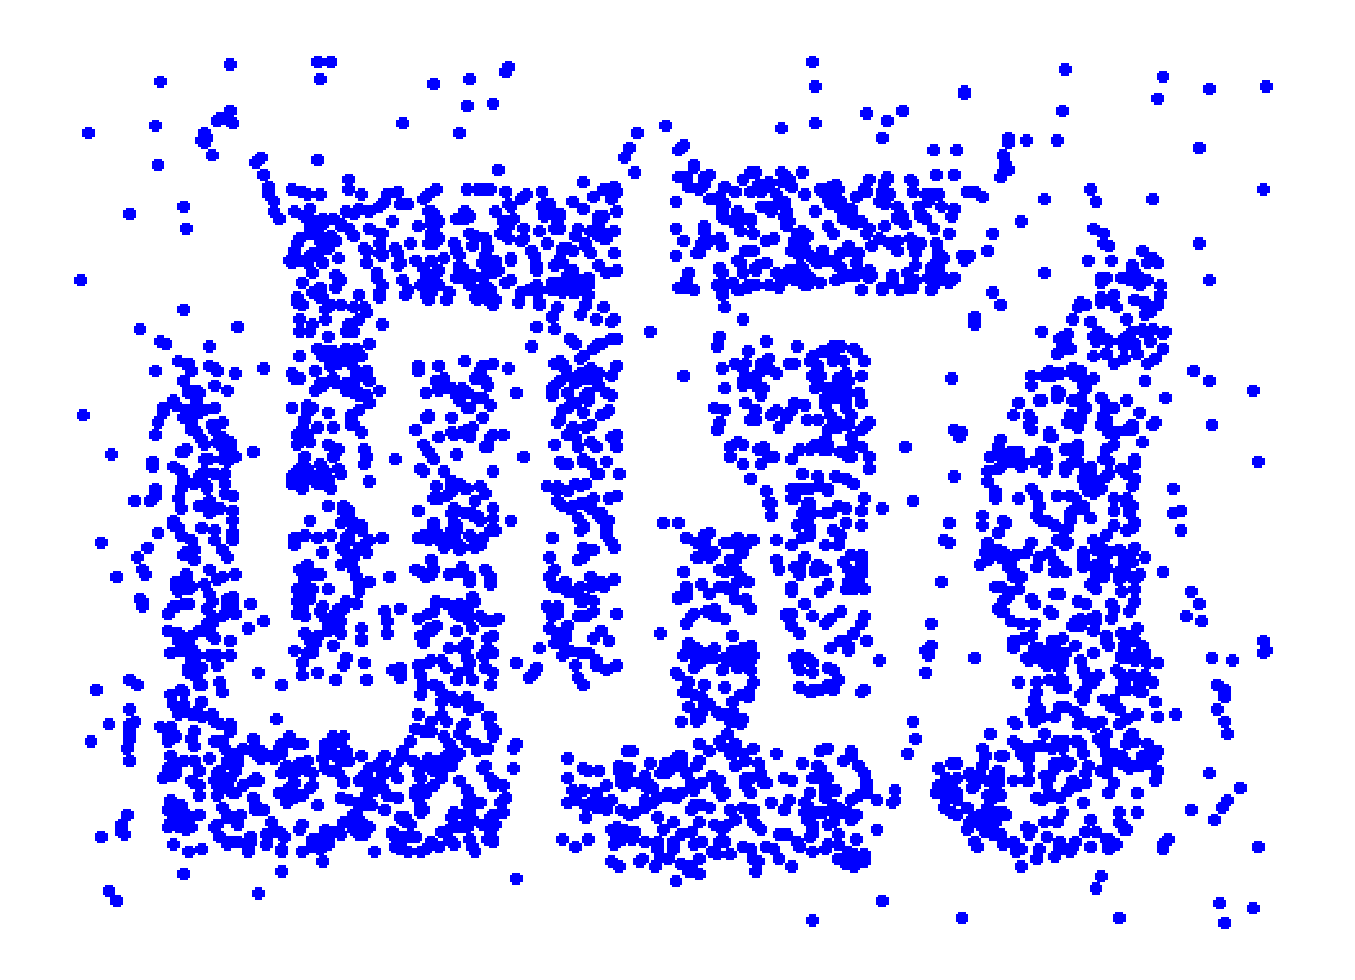
\includegraphics[width=\textwidth,height=4.0cm,keepaspectratio]{images/slide33_dbscan_reachability1.png}
      \end{center}
    \end{column}
    \begin{column}{0.48\textwidth}
      \begin{center}
        \textbf{خوشه‌های استخراج‌شده و نقاط نویز}\\[0.15cm]
        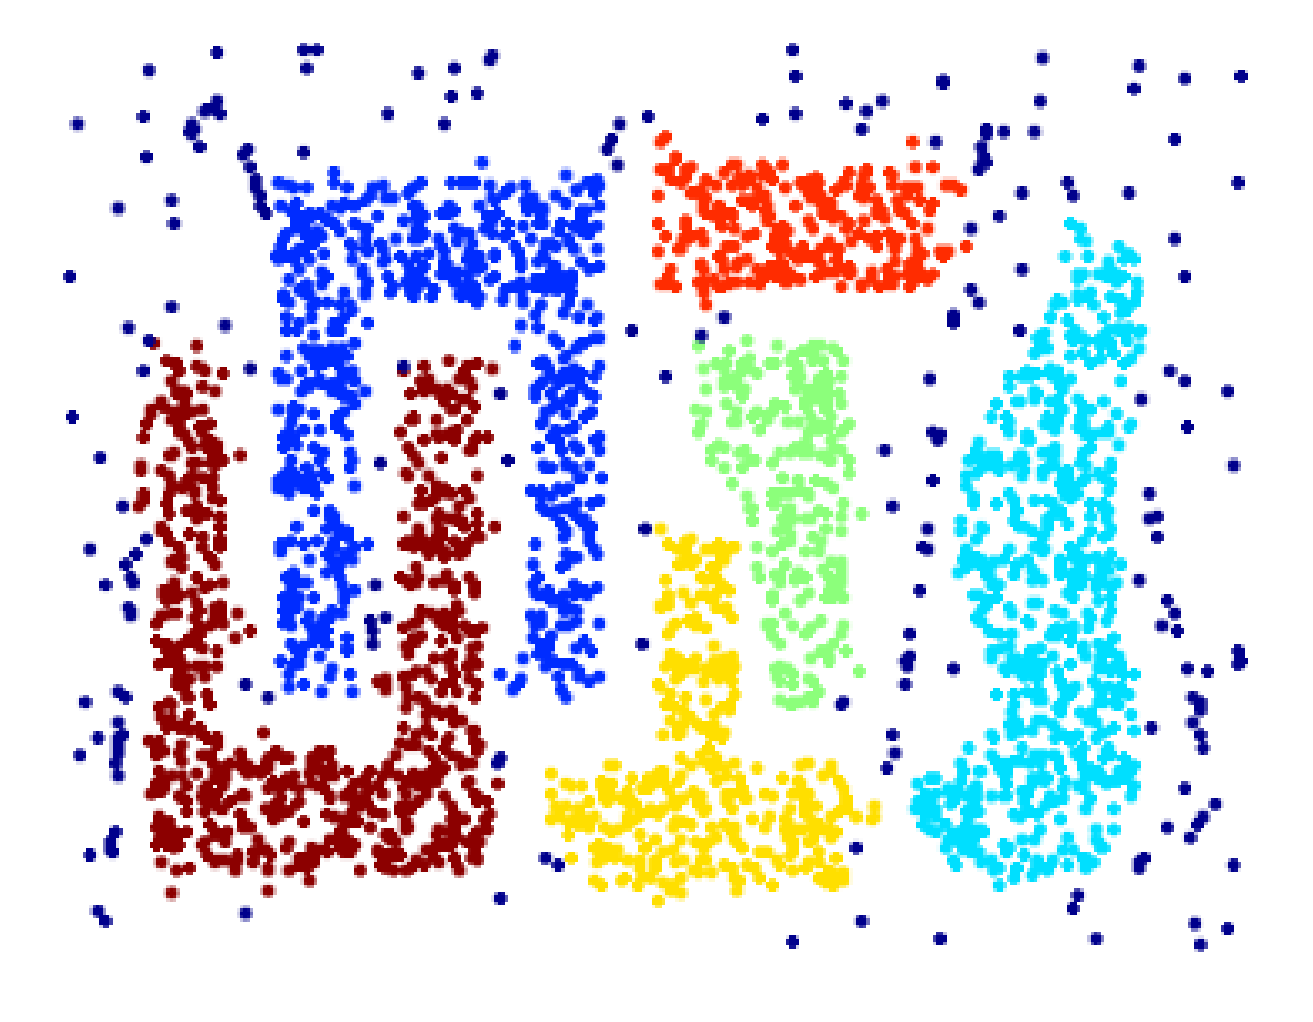
\includegraphics[width=\textwidth,height=4.0cm,keepaspectratio]{images/slide33_dbscan_reachability2.png}
      \end{center}
    \end{column}
  \end{columns}
\end{frame}

% Slide 34: When DBSCAN Does NOT Work Well
\begin{frame}{نقاط ضعف و چالش‌های \lr{DBSCAN}}{\lr{When DBSCAN Does NOT Work Well}}
  \begin{columns}[T]
    \begin{column}{0.4\textwidth}
      \begin{itemize}
        \setlength{\itemsep}{5pt}
        \item \textbf{چگالی‌های متغیر:} \lr{(Varying Densities)}
        \begin{itemize}
          \setlength{\itemsep}{2pt}
          \item با یک زوج $(\epsilon, \text{MinPts})$ ثابت نمی‌توان همزمان خوشه‌های با چگالی‌های متفاوت را تفکیک کرد.
          \item تغییر ناچیز $\epsilon$ خوشه‌ها را ادغام یا تجزیه می‌کند.
        \end{itemize}
        \item \textbf{داده‌های با ابعاد بالا:} \lr{(High-dimensional)}
        \begin{itemize}
          \setlength{\itemsep}{2pt}
          \item به دلیل نفرین ابعاد، فواصل یکنواخت شده و چگالی مفهوم خود را از دست می‌دهد.
        \end{itemize}
      \end{itemize}
    \end{column}
    \begin{column}{0.58\textwidth}
      \begin{center}
        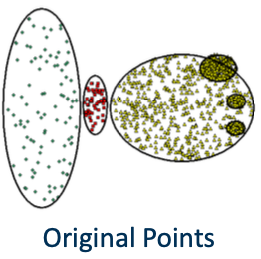
\includegraphics[width=0.48\textwidth,height=2.2cm,keepaspectratio]{images/slide34_density_original_user.png}\quad
        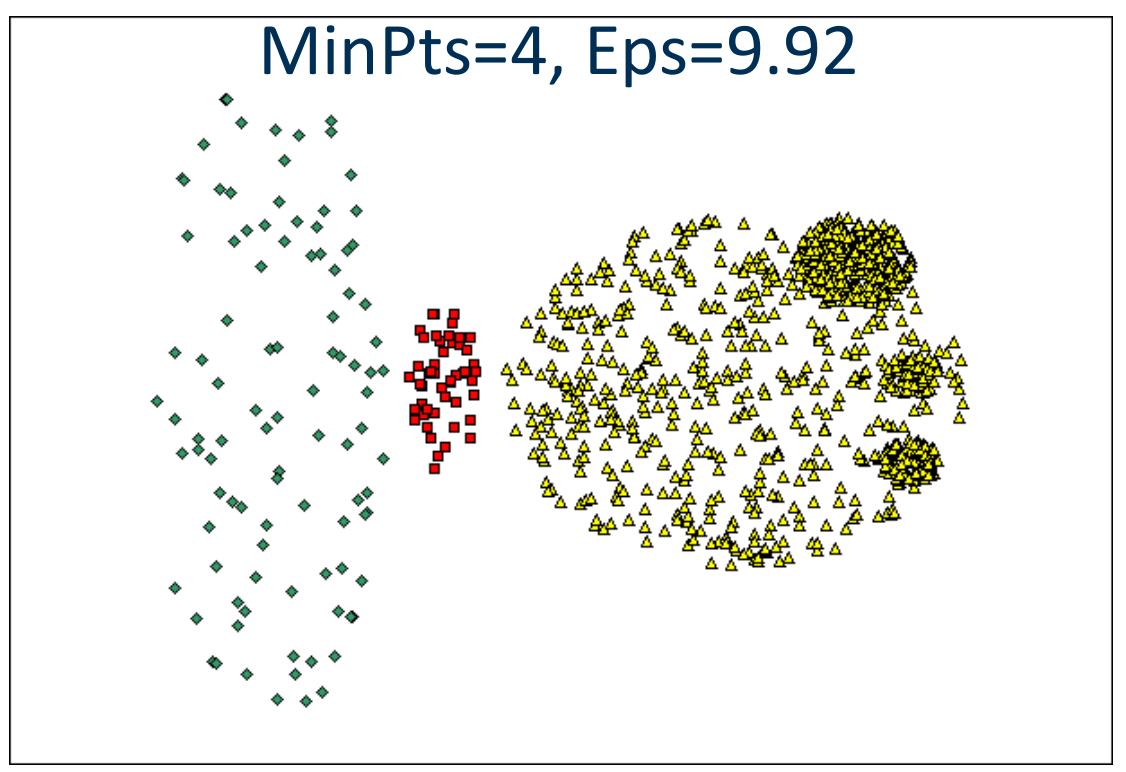
\includegraphics[width=0.48\textwidth,height=2.2cm,keepaspectratio]{images/slide34_dbscan_density2.png}\\[0.15cm]
        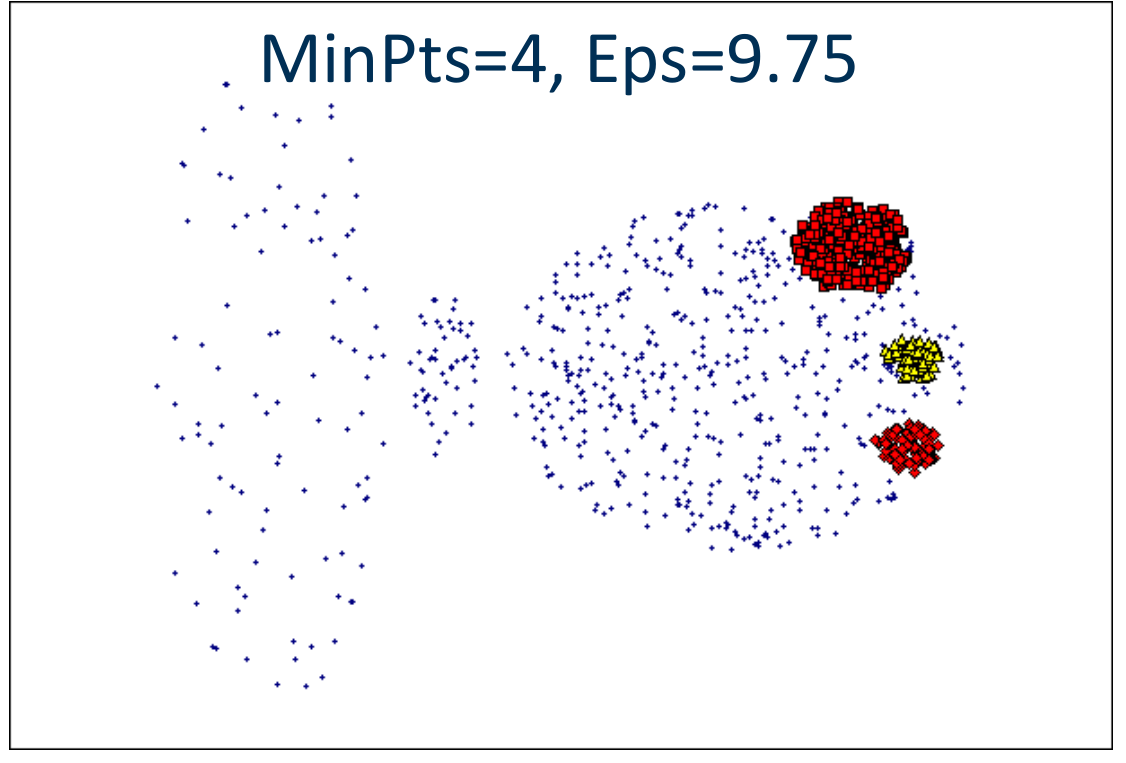
\includegraphics[width=0.58\textwidth,height=2.2cm,keepaspectratio]{images/slide34_dbscan_density3.png}
      \end{center}
    \end{column}
  \end{columns}
\end{frame}

% Slide 35: Determining EPS and MinPts
\begin{frame}{تعیین پارامترهای \lr{MinPts} و \lr{Eps}}{\lr{Determining EPS and MinPts}}
  \begin{columns}[T]
    \begin{column}{0.52\textwidth}
      \begin{itemize}
        \setlength{\itemsep}{5pt}
        \item \textbf{ایده اصلی:} برای نقاط درون یک خوشه، فاصله تا $k$-امین نزدیک‌ترین همسایه \lr{($k$-th Nearest Neighbor)} تقریباً یکسان است.
        \item نقاط نویز فاصله بسیار بزرگ‌تری تا $k$-امین همسایه خود دارند.
        \item \textbf{روش عملی:}
        \begin{itemize}
          \item محاسبه فاصله هر نقطه تا $k$-امین همسایه.
          \item مرتب‌سازی فواصل از کوچک به بزرگ و رسم نمودار.
          \item انتخاب مقدار $\epsilon$ در \textbf{نقطه زانو / شکست نمودار}.
        \end{itemize}
      \end{itemize}
    \end{column}
    \begin{column}{0.46\textwidth}
      \begin{center}
        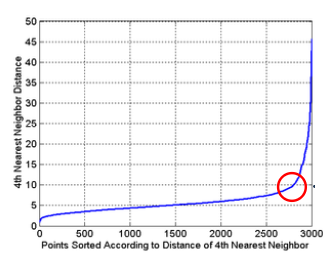
\includegraphics[width=\textwidth,height=4.5cm,keepaspectratio]{images/slide35_dbscan_kdist_user.png}
      \end{center}
    \end{column}
  \end{columns}
\end{frame}

% Slide 36: DBSCAN in Python
\begin{frame}{پیاده‌سازی الگوریتم \lr{DBSCAN} در پایتون}{\lr{DBSCAN in Python (Scikit-Learn)}}
  \begin{columns}[T]
    \begin{column}{0.56\textwidth}
      \begin{latin}
        \begin{minipage}{\textwidth}
          \fcolorbox{codeborder}{codebg}{%
            \begin{minipage}{0.96\textwidth}
              {\fontsize{7.0}{9.5}\selectfont\ttfamily
              \textcolor{mannheimteal}{\# 1. Import DBSCAN}\\
              \textcolor{blue}{\textbf{from}} sklearn.cluster \textcolor{blue}{\textbf{import}} DBSCAN\\[0.15cm]
              \textcolor{mannheimteal}{\# 2. Create the clusterer}\\
              clusterer = DBSCAN(\\
              \quad min\_samples=3,\\
              \quad eps=1.5,\\
              \quad metric=\textcolor{red}{'euclidean'}\\
              )\\[0.15cm]
              \textcolor{mannheimteal}{\# 3. Fit and predict clusters}\\
              clusters = clusterer.fit\_predict(\\
              \quad dataset[['Att1', 'Att2']]\\
              )
              }
            \end{minipage}%
          }
        \end{minipage}
      \end{latin}
    \end{column}
    \begin{column}{0.42\textwidth}
      {\fontsize{8.5}{11}\selectfont
      \textbf{پارامترهای کلیدی:}
      \begin{itemize}
        \setlength{\itemsep}{3pt}
        \item \codeinline{eps}: شعاع همسایگی ($\epsilon$).
        \item \codeinline{min\_samples}: حداقل تعداد نقاط درون شعاع \lr{(MinPts)}.
        \item \codeinline{metric}: تابع محاسبه فاصله (اقلیدسی، منهتن و ...).
      \end{itemize}
      \vspace{0.15cm}
      \textbf{نکته خروجی:}
      \begin{itemize}
        \item نقاطی که به عنوان نویز تشخیص داده شوند با برچسب \codeinline{-1} مشخص می‌گردند.
      \end{itemize}
      }
    \end{column}
  \end{columns}
\end{frame}
